%!TEX root = ../report.tex

\begin{document}
    \chapter{Methodology}

    \section{Pipeline Workflow: 2D Binary Lane Segmentation}
        \subsection{Architecture Overview}
        We have utilized the dual stage architecture proposed by \cite{guo2020gen} to obtain 3D lane points, where the output from the first stage is binary lane segmentation. And authors have not explored the efficacy of more complex architecture for binary 2D lane segmentation on 3D lane detection results. So we experimented with some mentioned approaches in section 3.1 for the same. In this section we will briefly discuss the neural network architecture for the binary 2D lane segmentation that we have experimented in this work. 
        
        Originally \cite{guo2020gen} have utilized ERFNet\cite{Romera2018ERFNetER} based network to obtain binary segmentation which is an auto-encoder based network for the first stage. For that we conducted a comaparative evaluation with the existing pretrained models using CondLaneNet\cite{DBLP:journals/corr/abs-2105-05003}, SCNN\cite{pan2018SCNN}, RESA\cite{DBLP:journals/corr/abs-2008-13719}, UFLD\cite{DBLP:journals/corr/abs-2004-11757}, LaneATT\cite{https://doi.org/10.48550/arxiv.2010.12035} which we will talk about in the later sections. As we have discussed in section 3.1 that there is more scope in extracting more meaningful features for segmentation based 2D lane detection and to facilitate the 3D lane detection we need 2D binary lane segmentation as an intermediate output. so explored two segmentation based approaches as mentioned above SCNN\cite{pan2018SCNN}, RESA\cite{DBLP:journals/corr/abs-2008-13719}. Both of these approaches are using semantic segmentation to predict 2D lane line points where the input to the network is a monocular image. But in out case we need binary segmentation as the output, so we modified the existing approaches to work for 2D binary lane segmentation.    
        
           \begin{figure}[h]
    \centering
    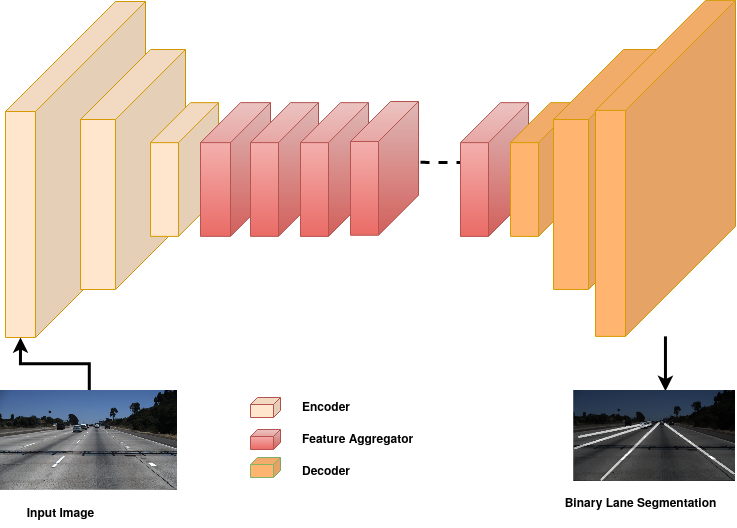
\includegraphics[width=12cm, height=7cm]{images/2dlane_pipleline.png}
    \caption{2D Binary Lane segmentation Pipeline}
    \end{figure}
        
        Figure 4.4 represents the pseudo architecture for the 2D binary lane detection module. This is an auto-encoder based pipeline where we have used ResNet \cite{DBLP:journals/corr/HeZRS15} based network for initial feature encoding and later utilizing the feature aggregation modules proposed by SCNN\cite{pan2018SCNN} and RESA\cite{DBLP:journals/corr/abs-2008-13719}. In the end we have experimented with two types of decoders for upsampling the extracted features as it is a dense prediction task we need the output to be of the same spatial size as input. Initially we used the a simple decoder proposed by SCNN\cite{pan2018SCNN} which uses bi-linear interpolation to upsample the feature maps, later we experimented with the Bilateral Upsampling Decoder (BUSD) proposed by RESA\cite{DBLP:journals/corr/abs-2008-13719}. So we trained our 2d binary lane segmentation pipeline using mix and match of the above mentioned encoder, decoder and feature aggregation modules.
        
        \subsection{Loss Functions Used}
        The task of semantic segmentation is considered as a dense prediction task, as the size of predictions and input remains same. The model predicts for every pixel a class label to which it belongs to. Binary segmentation can be seen as a subset of the task of semantic segmentation where instead of predicting multiple class labels we generally try to predict for the foreground and background. Foreground in our case can be the lane lines and background is the remaining entities in a driving scenario.
        Binary segmentation or semantic segmentation in general takes as an input a RGB image which can be of shape $(N,C,H,W)$ where $N$ is the batch size, $C$ the number of channels ie. in our case 3 representing $R, G, B$ and $H,W$ is the spatial size of the respective image. In case of binary segmentaiton the predictions are generally of the shape of $N,H,W$ or $N,C,H,W$ which later decides the choice of objective function used to train the pipeline. Binary Cross Entropy(BCE) is used in the case when the output is of the shape of $N,H,W$ as in the later case Cross Entropy is utilized.
        
                 \begin{figure}[h]
    \centering
    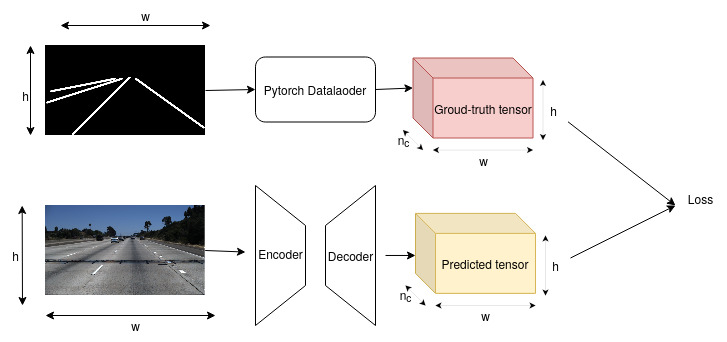
\includegraphics[width=13cm]{images/2d_dataflow_loss_computation.jpg}
    \caption{Data flow for loss computation for 2D binary lane segmentation pipeline. $w$ and $h$ are spatial width and height of the image tensors and $n_{c}$ represents the number of classes.}
    \end{figure}
        
        \subsubsection{Cross Entropy Loss}
        Cross Entropy is generally employed to measure the difference between two probability distributions.
        \begin{equation}
        L_{CCE} = -\frac{1}{N}\sum_{i=1}^{N} \sum^{M}_{j=1}y_{i,j}\cdot log(p_{i,j})
        \end{equation}
        
        where $p_{i,j}$ is the prediction for each class and $y_{i,j}$ is the target values for each class. $y_{i,j}$ is represented as one-hot encoded matrix of ground-truth labels which is represented in the form of different channels per each class. The rows and columns of each channels is either 0 or 1 depending upon the location of pixel-wise class labels. 
       
        \subsubsection{Focal Loss}
        Focal loss can be sen as an extened version of cross entropy where the objective function will penalise the hard samples than easy samples and to achieved that a regulating term is added to handle the class imbalance problem.
        \begin{equation}
            Cross Entropy = - \sum^{i=n}_{i=1}Y_{i}log_{b}(p_{i})
        \end{equation}
        where $Y$ is the ground-truth label and $p$ is the predicted probability.
        
        \begin{equation}
            Focal Loss = - \sum^{i=n}_{i=1} \alpha_{i}(1-p_{i})^{\gamma} log_{b}(p_{i})
        \end{equation}
        
         when $\gamma = 0$, Focal Loss is equal to Cross Entropy Loss. 
        
        \subsubsection{Dice Loss}
        Dice Similarity Coefficient(DSC) is a popular loss function which is used for the task of semantic segmentation to counter the problem of class imbalance. DSC is quite similar to Intersection over Union(IoU). Like IoU, Dice Similarity Coefficient(DSC) is used to compare the predicted segmentation mask and the corresponding ground truth. In simpler terms DSC is 2 times the area of overlap  between segmentation mask and ground-truth mask divided by the total number of pixels in both the prediction and ground-truth mask.
        
        \begin{equation}
            DC = \frac{2TP}{2TP + FP + FN} = \frac{2|X \cap Y|}{|X| + |Y|}
        \end{equation}
    where $TP$ are the true positivesm $FP$ false positives and $FN$ false negatives.  
        
        \begin{equation}
            L_{dice} = 1 - DSC
        \end{equation}
        
        \subsection{Evaluation Metrics}
        All the utilized datasets have their own evaluation metrics and even the authors have released the script for bench-marking the results and the evaluation criteria proposed by them only relies on penalizing the predictions on the basis of predicted 2d lane line points. As in our case we are not interested in predicting lane line points rather our 3D lane detection module relies on 2d binary lane segmentation masks as intermediate output. So we have used IoU (Intersection-over-union) or Jaccard Index to evaluate the trained models. IoU is a commonly used evaluation metric for image segmentation which is really effective. In Simple terms IoU calculated the area of overlap between the predicted segmentation mask and the ground truth divided by the union of the predicted segmentation mask and ground truth.
        
         \begin{figure}[h]
    \centering
    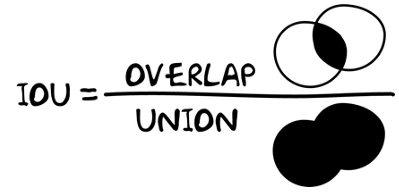
\includegraphics[width=7cm, height=4cm]{images/IOU.png}
    \caption{(IoU)Intersection-Over-Union \footnotemark}
    \end{figure}
    \footnotetext{\url{https://towardsdatascience.com/intersection-over-union-iou-calculation-for-evaluating-an-image-segmentation-model-8b22e2e84686}}
        
        \subsection{Implementation Details and Other Design Choices}
        We utilized three datasets for training the 2D binary lane segmentation pipeline. The first dataset is called TuSimple lane detection benchmark\cite{Tusimple}, as discussed in section 3.3.3 it is a simple dataset consists of normal highway driving. On the other hand we also use a more complex and much larger dataset compared to the previous one like CULane\cite{pan2018SCNN} which contains 55 hours of driving and contains different driving scenarios as discussed in section 3.3.3. We have also trained the 2D binay lane segmentation with Apollo Synthetic dataset\cite{guo2020gen} by utilizing the semantic segmentation labels provided in the dataset. We have conducted several experiments on the above mentioned datasets in terms of usage of different objective functions (dice loss, categorical cross entropy loss, focal loss), different variants of the network using mix and match of the above discussed encoder, decoders and feature aggregators. The input image is resized to $(360,480)$ and normalized using Imagenet\cite{deng2009imagenet} mean and standard deviation values. Adam\cite{Kingma2015AdamAM} with weight decay $1e-4$ is used as an optimizer to train our models. $0.001$ is chosen as an initial learning rate and on the top of that we have used ReduceLROnPlateu \footnote{\url{https://pytorch.org/docs/stable/generated/torch.optim.lr_scheduler.ReduceLROnPlateau.html#torch.optim.lr_scheduler.ReduceLROnPlateau}} as the learning rate scheduler with $0.75$ as learning rate reduction factor, $3$ as patience factor denotes the number of epochs to wait when the learning rate has to be reduced if there is no improvement in loss, $1e-6$ as the lowest learning rate manged by the scheduler. All the models are trained with the batch size of $8, 16$ but we have only reported the results with batch size $8$ and training is carried for $60$ epochs. During training, the model is evaluated at every epoch and the results are visualized qualitatively and quantitatively using wandb \footnote{\url{https://wandb.ai}}.
        
    %---------------------------------------------------------------- After here must start 3d lane detection section%   
        
        \section{Pipeline Workflow: 3D Lane Detection }
        Before delving into the approaches that we have used to obtain 3D lane line points we need to understand how a 3D lane is represented with respect to ego vehicle frame of reference and the anchor based representation of 3D lane curve.  
        
        \subsection{3D Lane Geometry}
        In this section we will introduce the geometric representation of lanes in 3D space, image plane and birds eye view via the means of the transformation from one space to another. 
        
         \begin{figure}[h]
    \centering
    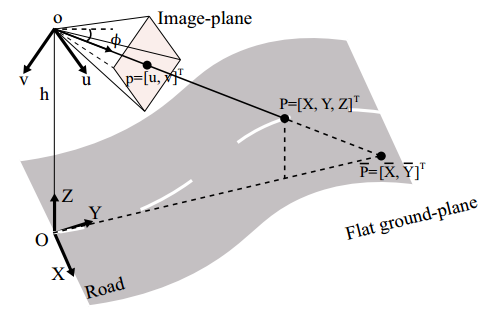
\includegraphics[width=9cm, height=5cm]{images/3d_lane_geometry.png}
    \caption{Geometric representation of lane point in 3D world space, image plane and virtual top view \cite{DBLP:journals/corr/abs-2112-15351}}
    \end{figure}
    
    In the above figure the point $\textbf{P} =[X, Y, Z]^{T}$ is in 3D space and when it is projected onto the image plane it is defined by $\textbf{p} = [u, v]^{T}$. Birds eye view can be seen as the projection of point $\textbf{P}$ from 3D space to flat ground plane, where $Z=0$. $\textbf{O}$ is the origin of the 3D space which is obtained by projecting the origin of camera center $\textbf{o}$ on to the flat ground plane with $Z = 0$. The focal length and other intrinsic parameters of the camera is fixed, where as the orientation of the camera in terms of camera height \textbf{h}  and camera pitch \textbf{$\phi$} is fixed or sometimes it is predicted from the network. 
    
    Using geometric transformation and homography as discussed above we can project points in 3D space to virtual flat ground plane. As per the figure 4.1 we can say that the point \textbf{P} it projection on image plane and flat ground plane, all lies on the same ray and this co-linear relationship will hold even if when there are downhill scenarios where $Z<0$. 
    
      \begin{figure}[h]
    \centering
    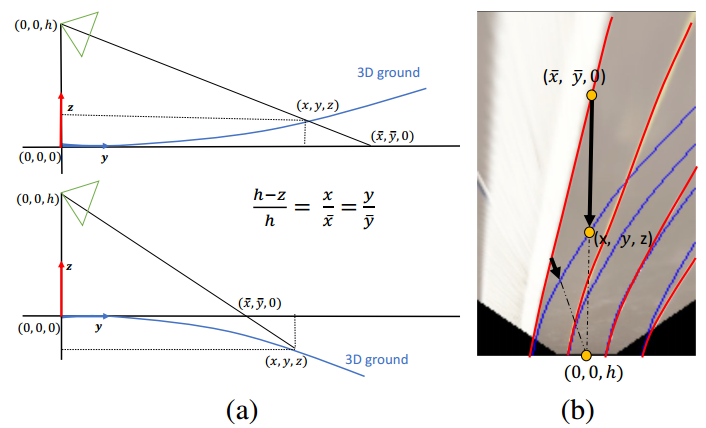
\includegraphics[width=9cm, height=5cm]{images/collinear_3dlane.png}
    \caption{Another view of the co-linear relationship between the 3D lane points $(x,y,z)$, its projection on virtual top view $(\overline{x}, \overline{y},0)$ and camera center $(0,0,h)$ \cite{guo2020gen}}
    \end{figure}

    Therefore we can obtain a relationship between the points from 3d world to virtual top view as :
    \begin{equation}
        \frac{h-z}{h} =\frac{x}{\overline{x}}=\frac{y}{\overline{y}} 
    \end{equation}
    
    using the above formulation we can represent this transformation from 3D world space to virtual top view as \textbf{$\overline{P} = GP$}, where \textbf{G} is the transformation matrix. Similarly a point \textbf{$\overline{P}$} can be projected onto the image plane as $\textbf{p}$ using homomgraphy which is also discussed in section 2.2. and this can be represented as: 
    \begin{equation}
       \begin{bmatrix}\overline{u}  \\\overline{v} \\ \overline{z}\end{bmatrix} = \begin{bmatrix} f_{x} & 0& c_{x}  \\0 &f_{x} & c_{y} \\ 0 & 0 & 1     \end{bmatrix}\begin{bmatrix} 1 & 0& 0  \\0 &cos(\phi+ \frac{\theta}{2}) & h \\ 0 &cos(\phi+ \frac{\theta}{2}) & 0     \end{bmatrix}\begin{bmatrix}\overline{X}  \\\overline{Y} \\ 1\end{bmatrix}
    \end{equation}

    Here, \textbf{$\widetilde{p}$} $= (\widetilde{u}, \widetilde{v}, \widetilde{z})$ and  \textbf{$\widetilde{P}$} $= (\overline{X},\overline{Y},1 )$ are represented in the form of homogeneous coordinates, therefore $u = \frac{\widetilde{u}} {\widetilde{z}} $ and $v = \frac{\widetilde{v}} {\widetilde{z}} $. Similar as above this can be represented as \textbf{$\widetilde{p} = H\widetilde{P}$}, where H is the homography transformation matrix. 
    
    \subsection{3D Lane Anchor Representation}
    Some of the approaches used in this work are predicting 3D lane line points in the from of anchors and even the ground-truth points are also converted in the form of anchors as target tensors to the network.  As per the 3D lane geometry discussed above, x is the lateral axes and Y is the forward axes with respect to a scene. These anchors are generally predefined on the basis of equally spaced distance in x and y directions. 
    
     \begin{figure}[h]
    \centering
    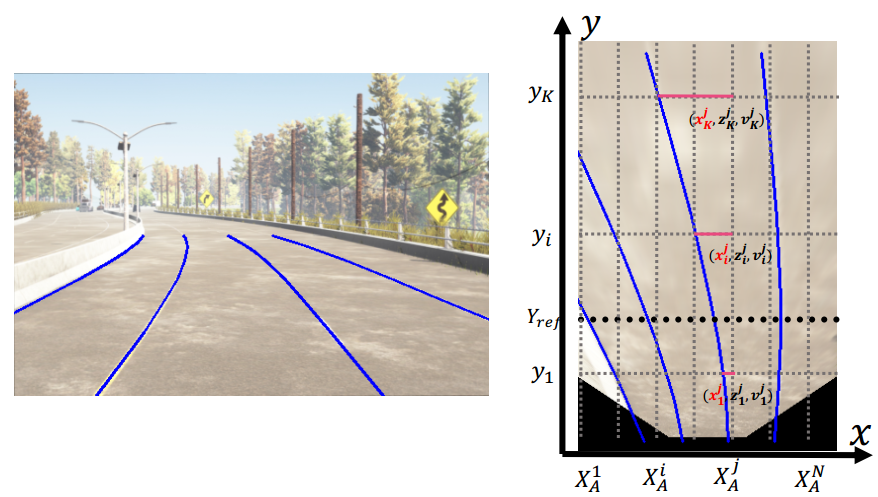
\includegraphics[width=9cm, height=5cm]{images/anchor_3Dlane.png}
    \caption{Lane anchor representation \cite{guo2020gen}}
    \end{figure}
    
    As per the figure 4.3, there exist N lane anchors (Vertical lines) in terms of N equally spaced position in X-direction ($X^{i}_{A}$)$^{N}_{i=1}$. The position on anchors in y-direction can be equally spaced or on the basis of certain distances in the forward direction. Therefore a 3D lane line in this can be represented by an anchor $X^{i}_{A}$ where each anchor contains $3*K$ attributes. K is the number of steps in y-direction. So at each step $(Y_ref)$ ground-truth lane anchor attributes ($\overline{x}^{i}_{j},z^{i}_{j},v^{i}_{j}$)$^{K}_{j=1}$ are calculated by associating it with the closest distance in x-direction. $\overline{x}^{i}_{j}$ are the horizontal offsets, $v^{i}_{j}$ is the visibility vector for every lane point.  In the later sections we will talk about the approaches that we have experimented with to obtain 3D lane line points. 
        
%--------------------------------Approach 1 starts from here::%        
        \subsection{Approach 1: GenLaneNet\cite{guo2020gen}}
        
        \subsubsection{Model Architecture Overview}
        Initially we have utilized the dual stage architecture proposed by \cite{guo2020gen} to obtain 3D lane points and later this dual stage way of architecture is used in our proposed 3D lane detection pipeline. In this section we will introduce the network architecture proposed by GenLaneNet\cite{guo2020gen} in detail and explain how we have utilized it for our initial experimentation for obtaining 3D lane line points.
        
         \begin{figure}[h]
    \centering
    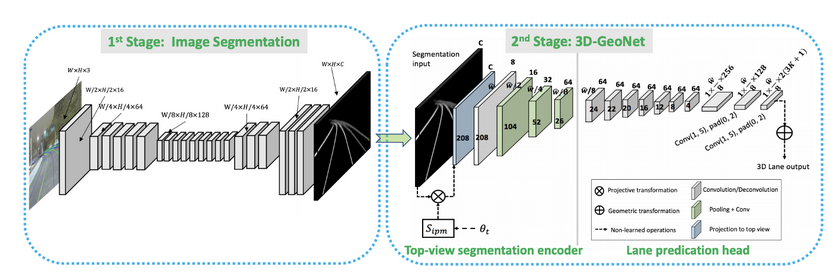
\includegraphics[width=13cm]{images/GenLaneNET.png}
    \caption{Network architecture of Gen-LaneNet \cite{guo2020gen}}
    \end{figure}
         
         Here authors have represented the 3D lane lines in the form of anchors and have utilized this representation to predict 3D lane line points by using a dual stage network. Authors have chosen this dual pathway approach on the fact that encoding 3D lane geometry is a different task to encoding features from image. Therefore, instead of predicting camera height and camera pitch the ground-truth values are used for obtaining all the geometric transformations. 
         The first stage is responsible for extracting features from the input monocular image and perform binary segmentation task on the image to obtain binary lane segmentation mask. This obtained binary lane segmentation mask is this used as an input for the next stage of the pipeline which is responsible for predicting the 3D lane line points in the form of anchor based representation. As described in section 4.2.2 each anchor defines a 3D lane line by 3*K values as ($\overline{x}^{i}_{j},z^{i}_{j},v^{i}_{j}$)$^{K}_{j=1}$. The ground truth target lane anchors are generated by taking the 3D lane line points which are in ego vehicle coordinate frame to virtual top view.
         
         The output from the image segmentation stage is processed by a top view segmentation encoder which uses projective transformation and project it into top-view which are further processed by a series of convolution layers to encode features from top view binary segmentation. After that a lane prediction head predicts 3D lane line points in terms of anchor representation. The predicted anchors are in top-view which can be further transformed into 3D lane line points in ego-vehicle frame by using geometric transformation. This dual stage network makes the pipeline flexible in terms of using complex binary segmentation solutions and make it affordable as we don't need more real world 3D lane lines labels in various driving scenarios.
        
        
        \subsection{Experimental Setup: Approach 1}
        
        
            \subsubsection{Loss Computation}
            While training, the pipeline takes as an input an RGB image and predicts an anchor based representation of 3D lane lines which is discussed in section 4.2.2. The ground-truth 3D lane points are projected in virtual top-view and the anchors are calculated in terms of different y-positions $\left\{ y_{i} \right\}^{k}_{j=1}$ by associating them with the closest anchors at that particular $Y_{ref}$. Loss function for the predicted anchors $\hat{X}_{A}^{i}$ and the ground-truth anchors $\hat{X}_{A}^{i}$ =$ \left\{(\hat{x^{i}_{t}},\hat{z^{i}_{t}},\hat{v^{i}_{t}},\hat{p^{i}_{t}})\right\}_{t\in\left\{c,l\right\}}     $ is defined as: 
            
            \begin{equation}% 
\mbox{\fontsize{15}{21.6}\selectfont\( %
 \begin{array}{l}
                l = - \sum_{t\in\left\{c,l\right\}} \sum ^{N}_{i=1}(\hat{p}^{i}_{t} logp^{i}_{t} + (1-\hat{p}^{i}_{t})log(1-p^{i}_{t}) )   \\ 
                +  \sum_{t\in\left\{c,l\right\}} \sum ^{N}_{i=1}\hat{p}^{i}_{t}\cdot(\parallel \hat{v}^{i}_{t} \cdot (x^{i}_{t} - \hat{x}^{i}_{t}) \parallel_{1} + \parallel \hat{v}^{i}_{t} \cdot (z^{i}_{t} - \hat{z}^{i}_{t}) \parallel_{1} ) \\ 
                + \sum_{t\in\left\{c,l\right\}} \sum ^{N}_{i=1} \hat{p}^{i}_{t} \cdot \parallel v^{i}_{t} - \hat{v}^{i}_{t} \parallel^{1}
            \end{array} %
\)} %
\end{equation}
            where $x^{i}_{t}$ represents the horizontal offset, $z^{i}_{t}$ indicates the height offset, $v^{i}_{t}$ denotes the visibility of lane points and $p^{i}_{t}$ is the probability of existence of a lane. 
        
            \subsubsection{Evaluation Metric}
            
            We have used the evaluation metric proposed by \cite{guo2020gen} which is defined as a bipartite matching problem between predicted lane anchors and ground-truth lane anchors. This bipartite matching is facilitated by calculating a pairwise cost between lane lines in terms of euclidean distance. 
        
            \subsubsection{Implementation Details and Other Design Choices}
        
%------------------------------------------------------------------------------------------ Approach 2 starts from here%
        \subsection{Approach 2}
        
        \subsubection{Architecture Overview of Proposed Dual Stage Semi-Local Anchor-Less 3D Lane Detection pipeline}
        
        Anchor based 3D lane detection approaches face similar challenges as anchor based 2D lane detection. Therefore it is not able to generalize well with different lane topologies. Utilizing the idea of dual stage network proposed by \cite{guo2020gen} and anchors less semi-local 3D lane detection approach proposed by \cite{DBLP:journals/corr/abs-2011-01535}, we proposed an semi-local anchor-less dual stage network for obtaining 3D lane line points.
        
        \begin{figure}[h]
    \centering
    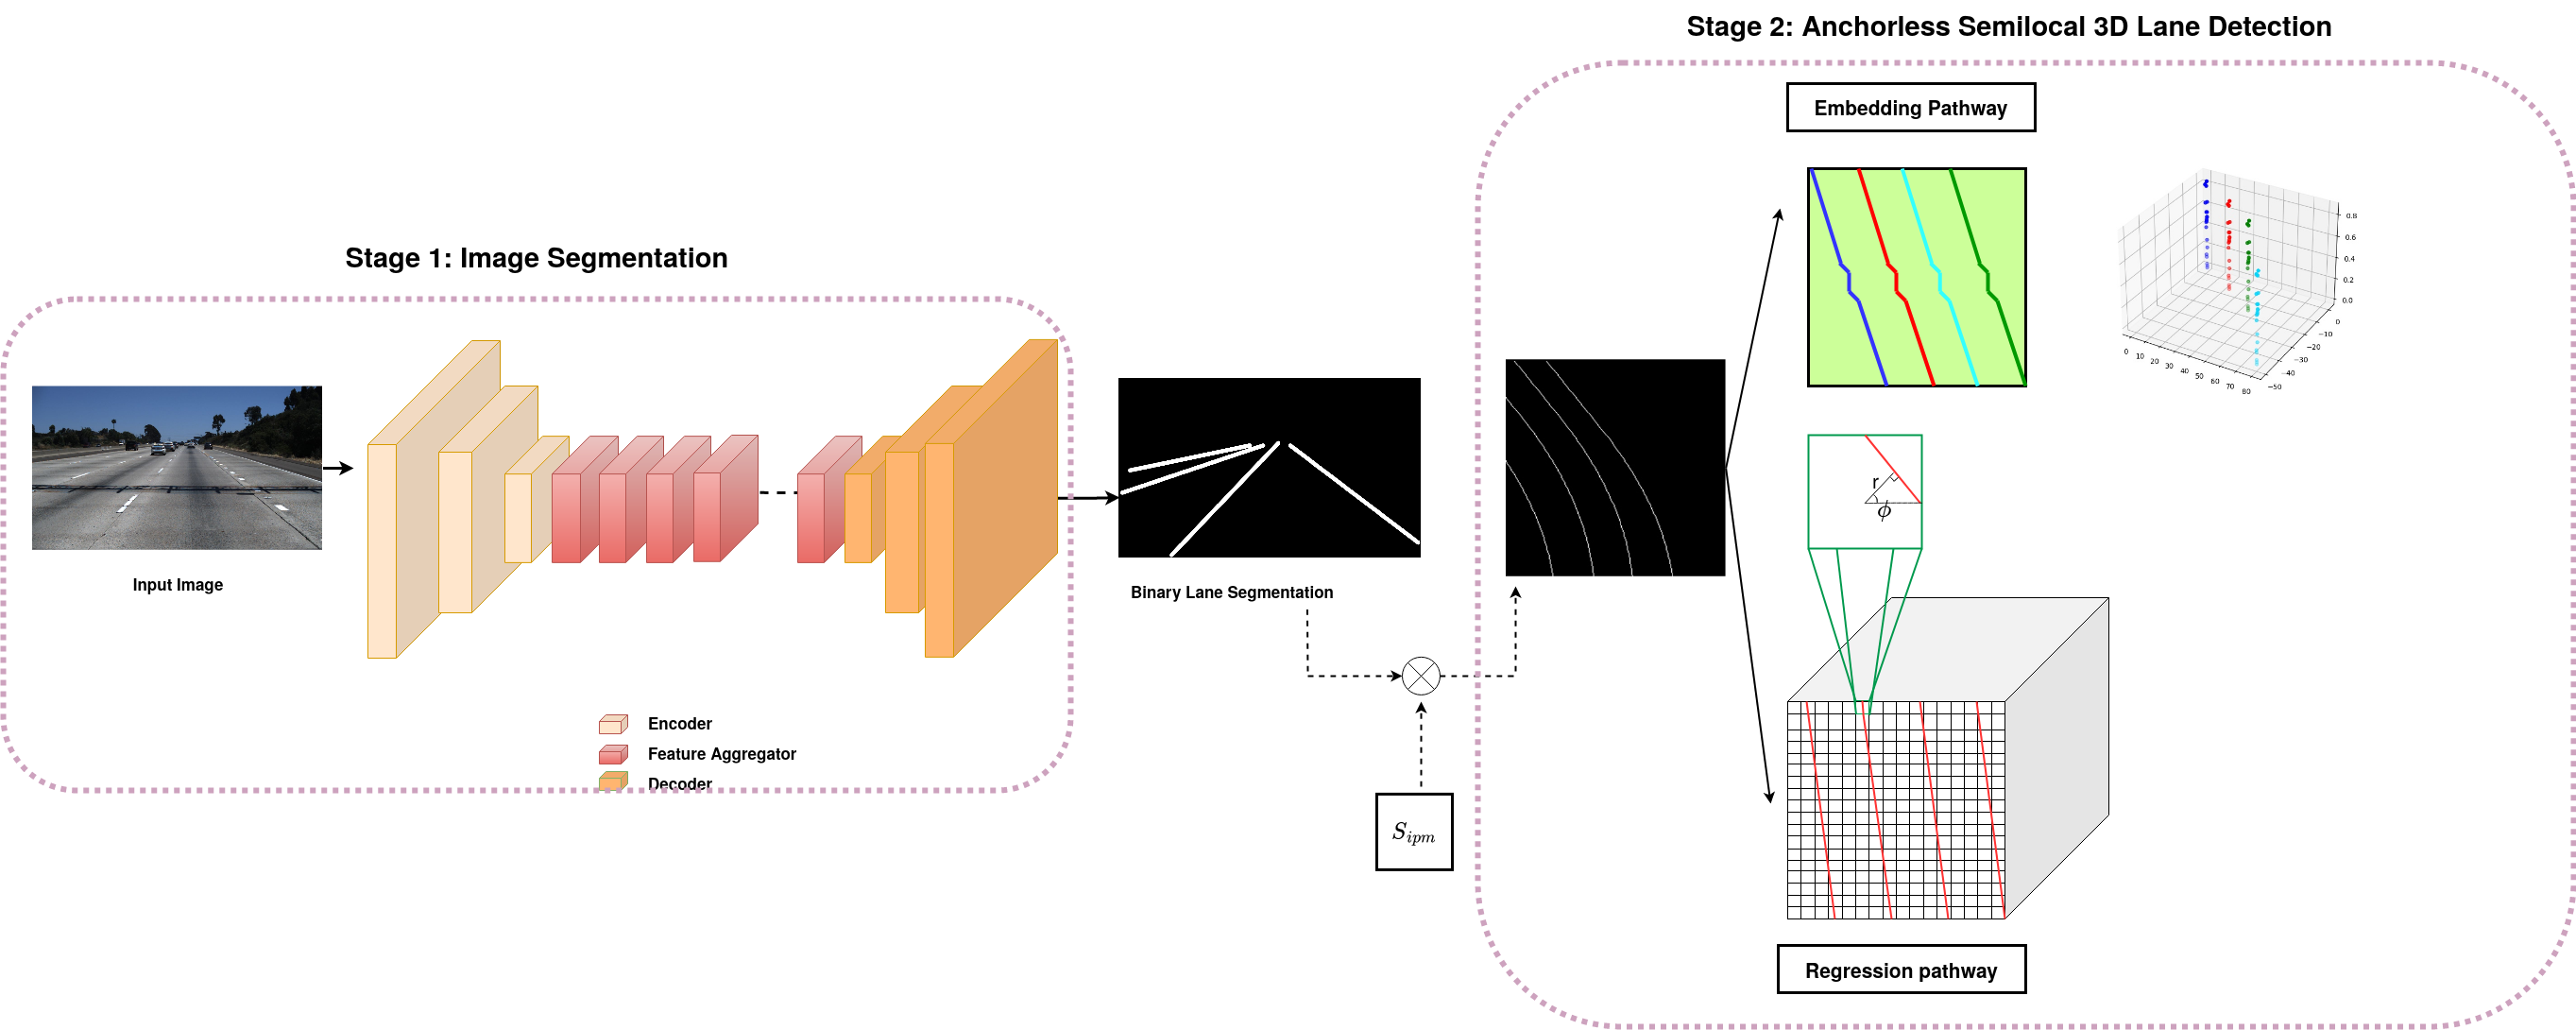
\includegraphics[width=\textwidth, height=7cm]{images/3DlaneAUXNet.png}
    \caption{Proposed dual stage semi-local anchor less 3D lane detection pipeline  \cite{guo2020gen}}
    \end{figure}
        
     As per the original idea of dual stage architecture proposed by \cite{guo2020gen}, the first stage is responsible for extracting features from a monocular image and obtaining binary lane segmentation mask as an intermediate output. This binary segmentation mask is taken into birds eye view using projective transformation. Before feeding the top-view binary lane segmentation mask into the second stage of the network it is normalized. Second stage of the network is divided into two pathways named as regression pathway and embedding pathway. Regression pathway is responsible for extracting geometric information for 3D lane curves. Inspired from \cite{DBLP:journals/corr/abs-2011-01535} we have used semi-local tile representation and predict the full lane curve by decimating the whole lane curve into small lane segments and regress geometric parameters to represent that lane curve locally. To facilitate that the resulting bird-eye-view feature map is spatially divided into grids $G_{WxH}$ containing $WxH$ non overlapping patches which are also called tiles. Assuming that from every tile there passes a line segment and approximating that line segment as a straight line, the regression pathway regresses per tile $g_{ij}$ three parameters ie. relative distance to tile center $\widetilde{r_{ij}}$, line angle $\widetilde{\phi_{ij}}$ and height offset $\triangle \widetilde{Z_{ij}}$. Instead of flattening the feature map and employ fully connected layers to predict regression targets for each tile, the output from the stage one is passed through a series of convolution layers which are processed in non-overlapping or semi-overlapping way where the kernel stride is set equal to the tile size and in the later case half of the tile size. Such encoding is responsible for regressing the geometric parameters for representing a lane segment per each tile, the spatial size of the output feature map after this encoding is same as $WxH$. Let's assume the spatial size of output birds eye view feature map after first stage is $(416,256)$ and diving this into a grid with each tile of size $(16,16)$, the resulting grid size will be $(26,16)$. Along with this the output size after the feature encoding is $(N, 13, H, W)$, here $(HxW) = (26x16)$ denoting the spatial size of the grid and $13$ denotes the number of channels for representing the tile regression targets which will be more explained in the later sections. Each element in this grid at a particular index along the channel axes represents the regression values for that particular tile. To generate the ground-truth regression targets for  angles and offsets the ground-truth lane points are projected into bird-eye-view and then approximating lane segments which passes through tile as straight lines. For this approximation bird-eye-view projected ground-truth lane points are divided into non overlapping grid and for each tile we have approximated the lane segments as straight lines using Hough transform which was introduced in section 2.3 
     
     In the embedding pathway the normalized birds-eye lane binary segmentation mask is fed to a series of $1x1$ convolution layers which is responsible for learning global lane embeddings, inspired by \cite{DBLP:journals/corr/abs-1802-05591} mean-shift clustering is performed on the learned global lane embedding to complete multiple lane segments to complete lane curves. We learn an embedding vector $f_{ij}$ for each tile and using discriminative push-pull loss inspired from \cite{DBLP:journals/corr/abs-2011-01535} \cite{DBLP:journals/corr/abs-1802-05591} as an objective function to learn the global lane embeddings. Discriminative push-pull loss ensures that the embedding that belong to the same line will stay close in the embedding space whereas embedding for tiles of different lanes will stay far from each other in embedding space. 

    \subsection{Experimental setup: Approach 2}
        \subsubsection{Dataset}
        
        \subsubsection{Loss Computation}
            \textbf{Rememember to mention the dataflow of the whole pipeline for the loss computation}
        
        \subsubsection{Evaluation Metrics}
        
        
        \subsubsection{Implementation Details}
            
            \textbf{<<<Explain the hyper params, design decisions(Tile size res, delta v delta d and more ), and experiments in-terms of tables for 3D lane detection>>>}
    
    \section{Pipeline Workflow: 3D Lane AuxNet}
        \subsection{Model Architecture}
        \subsection{Dataset}
        \subsection{Evaluation Metrics}
        \subsection{Implementation Details}
        
\end{document}
